\documentclass[a4paper]{article}


\usepackage{alphabeta} 
\usepackage{enumitem} 
\usepackage{mathtools}
\usepackage{amsmath, amssymb} 
\usepackage{amsthm}
\usepackage{cancel} 
\usepackage[margin=0.70in]{geometry} 
\geometry{left=2.9cm,right=3.0cm,top=2.1cm,bottom=2.3cm}	%the page geometry as defined, A4=210x297mm
\usepackage{graphicx}
\usepackage{wrapfig}
\usepackage{caption}
\usepackage{textcomp}
\usepackage{tabto}
\usepackage{layout}
\usepackage{bm}
\usepackage{minipage-marginpar}
\usepackage[dvipsnames]{xcolor}
\usepackage{hyperref}
\usepackage{dutchcal}
\usepackage{derivative}
\usepackage{esint}
%\usepackage{biblatex}
\usepackage{subcaption}
\usepackage{booktabs}\usepackage{derivative}
\usepackage[flushleft]{threeparttable}
\usepackage[capbesideposition=outside,capbesidesep=quad]{floatrow}
\usepackage{derivative}
\usepackage[thinc]{esdiff}
%%RENEW

\newtheorem{problem}{Άσκηση}
\newtheorem*{solution*}{Λύση}
\newtheorem{definition}{Ορισμός}[subsection]
\newtheorem{properties}{Ιδιότητες}[subsection]
\newtheorem{theorem}{Θεώρημα}[subsection]
\newtheorem{protash}{Πρόταση}[subsection]
\newtheorem{porisma}{Πόρισμα}[subsection]
\newtheorem{lemma}{Λήμμα}[subsection]
\newtheorem*{prooof}{Απόδειξη}
\newtheorem*{notes}{Παρατηρήσεις}
\newtheorem*{note}{Παρατήρηση}
\newtheorem*{app}{Εφαρμογή} 
\newtheorem*{example}{Παράδειγμα}
\newtheorem*{examples}{Παραδείγματα}


\newcommand\numberthis{\addtocounter{equation}{1}\tag{\theequation}}
%\renewcommand{\labelenumi}{\roman{enumi}}
\newcommand{\approxtext}[1]{\ensuremath{\stackrel{\text{#1}}{\approx}}}
\renewcommand{\figurename}{Εικόνα.}
\renewcommand{\tablename}{Πίνακας.}
%\renewcommand\refname{New References Header}
\renewcommand*\contentsname{Περιεχόμενα}
%\DeclareDerivative{\odv}{\mathrm{d}}


\begin{document}
\begin{titlepage}			%makes a title page. Remember to change the author, CID, username and group number to what is appropriate for you!
	\centering
	{\scshape\LARGE Εθνικό Μετσόβιο Πολυτεχνείο\par}
	{\scshape \LARGE Σ.Ε.Μ.Φ.Ε.\par}
	\vspace{1cm}
	{\huge\bfseries Συμβολομετρία \par}
	\vspace{1cm}
	{\Large\itshape Θωμόπουλος Σπύρος\par}		%remember to change these!
	
	%		{\large Group \@group\unskip\strut\par}
	{\large A.M ge19042 \hfill \\ E-mail spyros.thomop@gmail.com \\}%ge19042@mail.ntua.gr\par		%remember to change these!
	\vspace{1cm}
	{\large Ημερμονηνία Παράδοσης 07/01/2022\par}
\end{titlepage}


\newpage 

\subsection*{Συμβολόμετρο Michelson}

Μία δέσμη φωτός εκπέμπεται απ' την πηγή laser (Π) και προσπίπτωντας στο ημιδιαπερατό κάτοπτρο ΔΔ διαχωρίζεται στα δύο, μία ανακλώμενη που κατευθύνεται προς το κάτοπτρο ΚΚ και μία διαθλώμενη που κατευθύνεται προς το ΣΚ. Οι δύο δέσμες  συμβάλλουν στην τελική δέσμη σ. Η συμβολή μπορεί να είναι ενισχυτική είτε αναιρετική ανάλογα με την διαφορά δρόμου τους δ. Πιό συγκεκριμένα: 
\begin{align*}
\text{Ενισχυτική:\textcolor{white}{....}} \delta = m\lambda/2, |m|=1,3,5,...\numberthis\\
\text{Αναιρετική:\textcolor{white}{....}} \delta = m\lambda/2, |m|=0,2,4,...
\end{align*}
Αυτό ισχύει αν τα δύο κάτοπτρα είναι σταθερά, όμως στην περίπτωσή μας το ΚΚ κινείται με ταχύητα $v$ και ως συνέπεια τα μέγιστα της έντασης των δεσμών που συμβάλλουν αλλάζουν συνεχώς σε ελάχιστα και αντιστρόφως. Υπάρχει δηλαδή μία συχνότητα εναλλαγής μεγίστου-ελαχίστου ίση με 
\begin{align*}
\Delta f = \frac{2v}{\lambda}
\end{align*}
Προσθέτωντας έναν φακό Φ1 εμπρός του laser κάνουμε την δέσμη κωνική και στην εικόνα συμβολής παρατηρούμε φωτεινούς και σκοτεινούς δασκυτλίους. Έτσι αν $\beta_m$ η γωνία που αποκλίνουν οι δέσμες που προσπίπτουν στο κινούμενο κάτοπτρο, τότε οι συνθήκες ενίσχυσης-απόσβεσης γίνονται: 
\begin{align*}
\text{Ενισχυτική:\textcolor{white}{....}} 4xcos\beta_m = m\lambda, |m|=1,3,5... \numberthis \\
\text{Αναιρετική:\textcolor{white}{....}}4xcos\beta_m = m\lambda, |m|=0,2,4,... \numberthis
\end{align*}
Όπου $x=\delta/2$.


\begin{figure}[h!]
\centering
\caption{ Διάταξη Συμβολομέτρου Michelson}
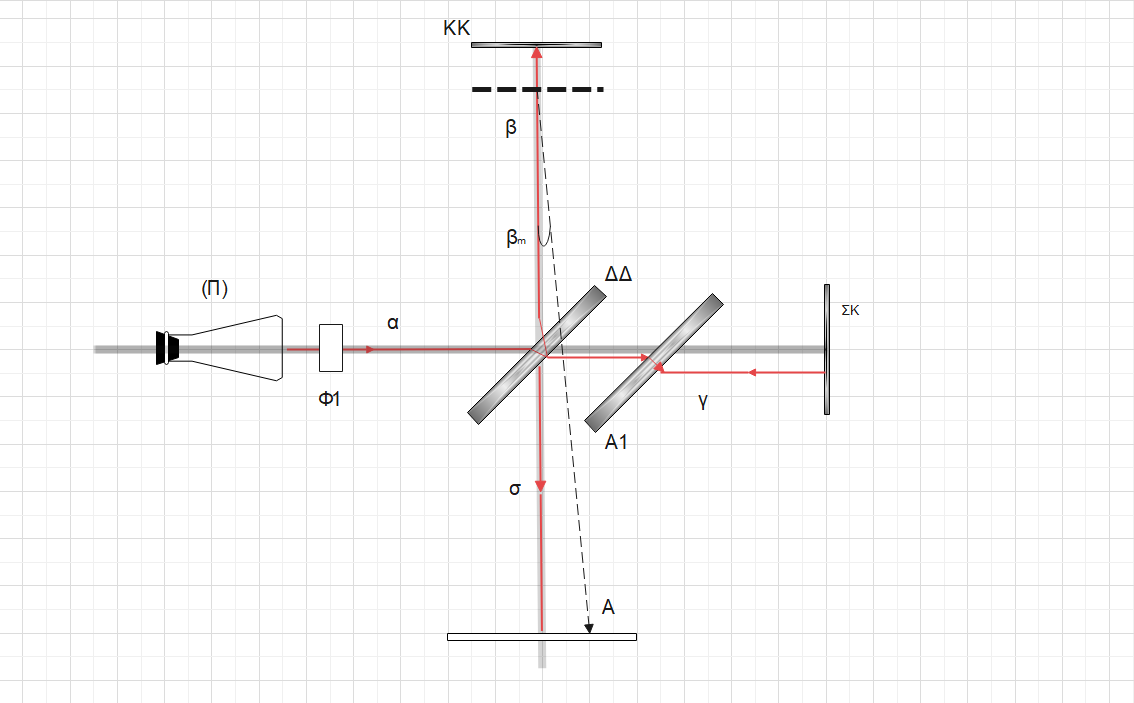
\includegraphics[scale=0.5]{michelson.png}
\end{figure}

Αφού ευθυγραμμίσουμε την ανακλώμενη δέσμη απ' το ΚΚ έτσι ώστε να επιστρέφει ακριβώς πάνω στην αρχική πηγή laser θα πρέπει στον τοίχο Α να παρατηρούμε κυκλικούς κροσσούς. Καταγράφουμε την θέση του μικρομετρικού κοχλία, θέτουμε σε λειτουργία το μοτέρ και παρατηρούμε να δημιουργούνται διαρκώς νέοι κροσσοί. Αφού μετρήσουμε 100 νέους κροσσούς ενίσχυσης ξαναμετράμε την ένδειξη του μικρομετρικού κοχλία και σημειώνουμε την διαφορά της αρχικής με την τελική ένδειξη. 

Έπειτα, χρησιμοποιώντας την σχέση (1) λυμένη ως προς $\lambda$ υπολογίζουμε το μήκος κύματος και το αντίστοιχο σφάλμα από την διάδοση των σφαλμάτων της μέτρησης στον μικρομετρικό κοχλία και των κροσσών.
Τα αποτελέσματα φαίνονται στον Πίνακα 1 .


\newpage


\begin{table}[h!]
\centering
\caption{ }
\begin{tabular}{r|r|r|r}
$\Delta x(\pm0.001mm)$ & $m(\pm2 \#\text{κροσσών})$  & $\lambda (\mathring{A})$ & $\Delta\lambda(\mathring{A})$ \\ 
\hline\hline
0.017 & 100 & 6800 & 423\\ 
0.016 & 100 &	 6400 & 420\\
0.015 & 100 & 6000 & 418\\ 
0.016 & 100 & 6400 & 420\\ 
0.017 & 100 & 6800 & 423\\
\end{tabular}
\end{table}

Εν τέλει η μέση τιμή του μήκους κύματος και το αντίστοιχο σφάλμα της είναι
\begin{align*}
\lambda = ( 6480\pm 335) \mathring{A}
\end{align*}
Παρατηρώ πως η τιμή συμπίπτει εντός των ορίων του σφάλματος με την αναμενόμενη των $6328\mathring{A}$.


\subsection*{Συμβολόμετρο Fabry-Perot}

\begin{wrapfigure}{r}{0.4\textwidth}
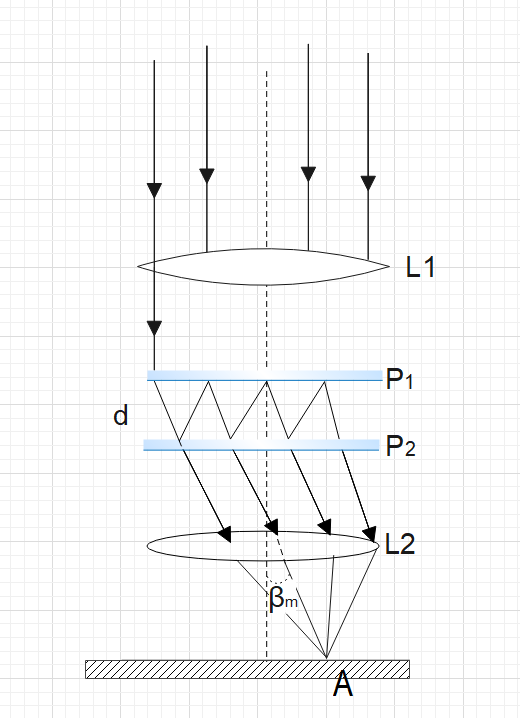
\includegraphics[width=0.7\linewidth]{fabry.png} 
\caption{ Αρχή Λειτουργίας Fabry-Perot}
\label{fig:wrapfig}
\end{wrapfigure}

Η διάταξη του συμβολομέτρου Fabry-Perot	 φαίνεται στην Εικόνα 2.
 Μία δέσμη laser γίνεται κωνική περώντας από τον φακό L1 και έπειτα εισέρχεται στην περιοχή με τα δύο ημιδιαφανή κάτοπτρα που απέχουν απόσταση d. Καθώς εισέρχεται, κάθε φορά που προσπίπτει στο Ρ2 ένα μέρος της διέρχεται από αυτό και όλα εστιάζουν, διερχόμενα από έναν φακό L2 σε κάποιο σημείο Α μίας οθόνης (στην περίπτωσή μας στον τοίχο).
Εξ' αιτίας της διαφοράς φάσης του κάθε διαθλώμενου μερους της ακτίνας, το αποτέλεσμα στο Α θα είναι ενισχυτική ή ακυρωτική συμβολή. Συγκεκριμένα θα δημιουργούνται πάλι σκοτεινοί και φωτεινοί κροσσοί συμβολής όπως και στην περίπτωση του συμβολομέτρου Michelson και θα ισχύουν οι σχέσεις (2) και (3) βάζοντας στο αριστερό μέρος έναν παράγοντα για τον δείκτη διάθλασης n του μέσου που βρίσκεται ενδιάμεσα των κατόπτρων.

Η ένταση στα σημεία συμβολής εξαρτάται από την διαφορά φάσης 
\begin{align*}
\Delta_m = \frac{4\pi n d cos(\beta_m)}{\lambda}
\end{align*}
όπου $\beta_m$ η γωνιακή απόκλιση του κροσσού m τάξης.

Αφού συναρμολογηθεί η διάταξη, θέτουμε σε λειτουργία το μοτέρ το οποίο μεταβάλλει την απόσταση των δύο κατόπτρων Ρ1, Ρ2 και συνεπώς αλλάζει διαρκώς τον κεντρικό κροσσό από φωτεινό σε σκοτεινό. Εμείς μετράμε τον χρόνο που απαιτείται για να γίνουν 100 τέτοιες εναλλαγές. Τα αποτελέσματα για 5 μετρήσεις φαίνονται στον Πίνακα 2. 

\begin{table}[h!]
\centering
\caption{ }
\begin{tabular}{r|r|r|r|r|r}
$\Delta t(\pm0.5sec)$ & $m(\pm2 \#\text{κροσσών})$  & $\Delta f (Hz)$ & $\delta\Delta f(Hz)$ & $u(10^{-6}m/s)$ & $\delta u(10^{-6}m/s)$ \\ 
\hline\hline
51.0 & 100 & 1.961 & 0.044 & 0.62 & 0.01\\
51.2 & 100 & 1.953 & 0.044 & 0.62 & 0.01\\
51.0 & 100 & 1.961 & 0.044 & 0.62 & 0.01\\ 
51.6 & 100 & 1.938 & 0.043 & 0.61 & 0.01\\
51.8 & 100 & 1.931 & 0.043 & 0.61 & 0.01\\
\end{tabular}
\end{table}
Οι στήλες 3-6 προκύπτουν από τις παρακάτω σχέσεις
\begin{align*}
\Delta f       &= m / \Delta t \\ 
\delta\Delta f &= \sqrt{\left(\pdv{\Delta f}{m} \delta m\right)^2 +\left( \pdv{\Delta f}{\Delta t} \delta\Delta t\right)^2} =  \frac{1}{\Delta t}\sqrt{\left(\delta m\right)^2 +\left( \frac{m}{\Delta t}\delta\Delta t \right)^2  } \\ 
u &= \lambda \Delta f  /2, \text{ για 0$\lambda=6328\mathring{A}$} \\ 
\delta u &= \sqrt{\left(\pdv{u}{\Delta f}\delta\Delta f \right)^2 } = \frac{\lambda}{2}\delta\Delta f
 %+\left(\pdv{u}{\lambda}\delta\lambda \right)^2 } } = 
\end{align*}

Η μέση τιμή της συχνότητας εναλλαγής του κεντρικού κροσσού είναι 
\begin{align*}
\Delta f = (1.949\pm0.014)Hz
\end{align*}
ενώ για την ταχύτητα του κινούμενου κατόπτρου
\begin{align*}
u = (0.62\pm0.01)\times10^{-6}m/s
\end{align*}
\subsection*{Γενικά}
Μερικές εφαρμογές για τα παραπάνω συμβολόμετρα είναι (Michelson$\rightarrow M$, Fabry-Perot$\rightarrow$ FP).

\subsubsection*{Συμβολόμετρο Michelson}

\begin{wrapfigure}{r}{0.4\textwidth}
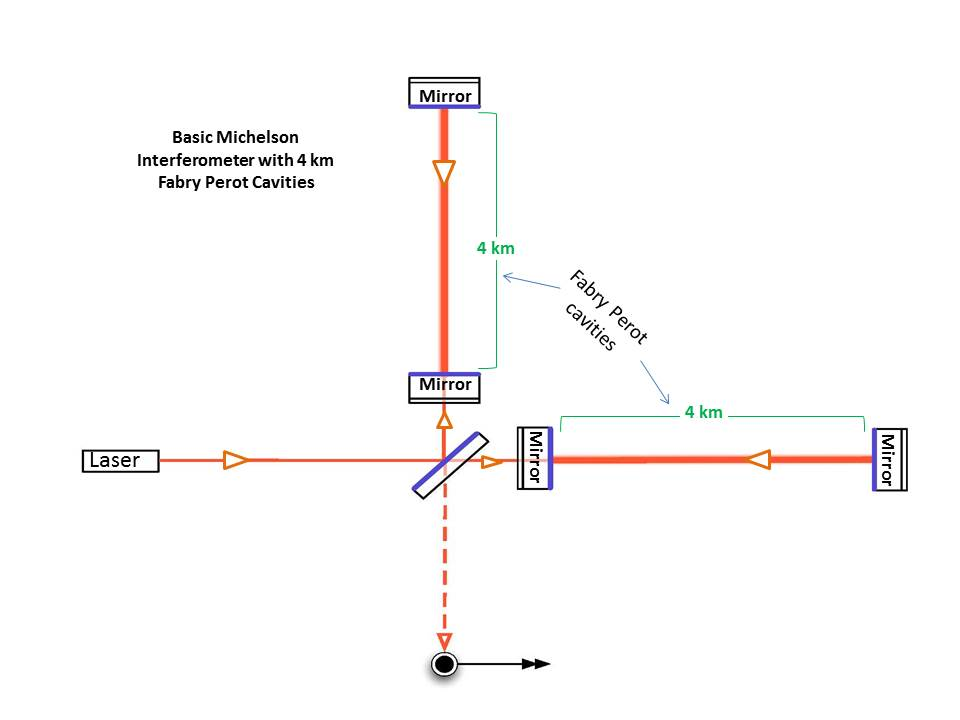
\includegraphics[width=0.8\linewidth]{ligo.jpg} 
\caption{ LIGO Fabry-Perot}
\label{fig:wrapfig}
\end{wrapfigure}
\textbf{(I. M/FP)} Η πίο εντυπωσιακή εφαρμογή των παραπάνω συμβολομέτρων θεωρώ πως είναι η χρήση τους για την ανίχνευση βαρυτικών κυμάτων στα πειράματα LIGO/VIRGO.
 Εκεί οι αποστάσεις των βραχιόνων είναι στα 4km. Καθώς ένα βαρυτικό κύμα περνάει από την περιοχή που υπάρχει ένα τέτοιο συμβολόμετρο στρεβλώνει τον χώρο γύρω του και ως εκτούτου μεταβάλλεται το μήκος των βραχιόνων.
	 Έτσι η ένταση των συμβαλλόμενων δεσμών μεταβάλλεται, αφού μεταβάλλεται η απόσταση που διανύει η κάθε δέσμη, και από αυτή την μεταβολή, αποκόπτοντας φυσικά τον εξωτερικό θόρυβο, μπορούν όχι μόνο να ανιχνεύσουν τα βαρυτικά κύματα αλλά επιπλέον να προσδιορίσουν και την πηγή τους (σύγκρουση μαύρων τρυπών, αστέρων νετρονίων κλπ). 
	
	Η διαφορά των αποστάσεων που προκαλούν τα βαρυτικά κύματα είναι της τάξης των $10^{-18}m$ την οποία και ανιχνεύουν. Ωστόσο στοχεύουν σε περεταίρω βελτίωση της διακριτικής ικανότητας και αντιμετωπίζουν προβλήματα/περιορισμούς όπως το shot-Poisson noise που οφείλεται στην τυχαία παραγωγή φωτονίων απ' το laser ή τον θερμικό θόρυβο εξαιτίας της κίνησης Brown και άλλους μη σταθερούς θορύβους όπως περιβαλλοντικές δονήσεις-σεισμούς.
	
Αρχικά είχε χρηιμοποιηθεί συμβολόμτρο Michelson αλλά προστέθηκαν δύο κάτοπτρα στους βραχίονες των 4km με αποτέλεσμα η δέσμη να ανακλάται $\sim300$ φορές πριν εξέλθει από αυτόν. Έτσι βελτιώνεται η ευθαισθησία. 

\textbf{(II. M)} Βρίσκει εφαρμογή στην τεχνική \textit{Shareography}, η οποία χρησιμοποιείται ευρέως στον μη-καταστροφικό έλεγχο υλικών στην αεροδιαστημική επίστήμη, με την οποία συλλέγουν πληροφορίες για το πως συμπεριφέρεται το υλικό σε ανάλογα με τις διάφορες εσωτερικές του μηχανικές τάσεις.
 Συγκεκριμένα, στην εν λόγω εφαρμογή, με το συμβολόμετρο Michelson μετράνε την διαφορά φάσης μίας δέσμης laser He-Ne (μήκους κύματος $632.8nm$) εξαιτίας της πρόσπτωσής της στην επιφάνεια ενός υλικού που έχει παραλάβει καθορισμένα φορτία.

(\textbf{III. M})  Μπορούμε να μετρήσουμε τον \textit{δείκτη διάθλασης} ενός υλικού. Παραδείγματος χάριν, αν τοποθετήσουμε ένα πλακίδιο, γνωστού πάχους L και αγνώστου δείκτη διάθλασης n, στην διαδρομή της μίας δέσμης τότε θα ισχύει  η σχέση  
\begin{align*}
L(n-1) = \frac{\Delta m\lambda}{2}
\end{align*}
Έτσι για καθορισμένο $\Delta m$, γνωστα L και λ, μπορούμε να υπολογίσουμε τον δείκτη διάθλασης.
\newpage
(\textbf{IV. FP})
 Χρησιμοποιείται για την ανίχνευση μεθανίου στον Άρη 
 \begin{wrapfigure}{r}{0.4\textwidth}
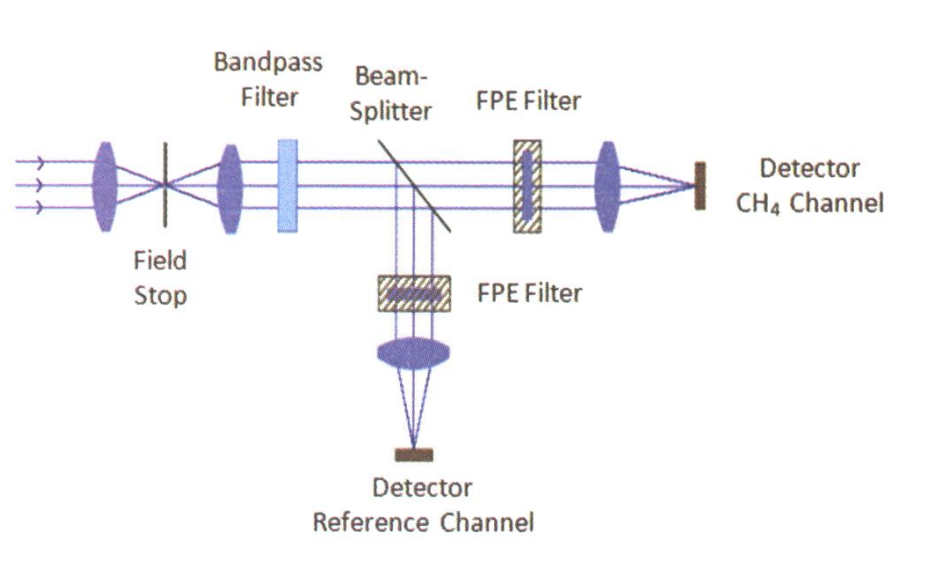
\includegraphics[width=0.8\linewidth]{methane sensor mars.png} 
\caption{Βασική Διάταξη του Methane Sensor for Mars}
\end{wrapfigure}
και την μέτρηση της συγκέντρωσής του. Είναι σχεδιασμένο έτσι ώστε να εμφανίζει μέγιστα διάδοσης της ακτινοβολίας από αυτό, σε σημεία τέτοια ώστε να συμπίπτουν με τα 6 μήκη κύματος απορρόφησης του μεθανίου. Η ακτινοβολία προέρχεται από ανάκλαση στην επιφάνεια του Άρη και εν συνεχεία καθώς διασχίσει το συμβολόμετρο Fabry-Perot καταλήγει σε έναν αισθητήρα. Έτσι υπάρχει η δυνατότητα μέτρησης διαφορετικής συγκέντωσης μεθανίου, η οποία υπολογίστηκε για συνήθεις συνθήκες πίεσης και θερμοκρασίας στον Άρη, περίπου ίση με $50ppb$.

Το εν λόγω ερώτημα ενδιαφέρει πολύ, καθώς η ακριβής μέτρηση της συγκέντρωσης ενδεχωμένως να δείνει ενδείξεις για την ύπαρξη ζωής στον Άρη κάποια περίοδο του παρελθόντος ή ακόμη και στο παρόν, αλλά σε μικροβιακή μορφή.
%\begin{wrapfigure}{r}{0.4\textwidth}
%\centering
%\caption{ Βασική Διάταξη του Methane Sensor for Mars}
%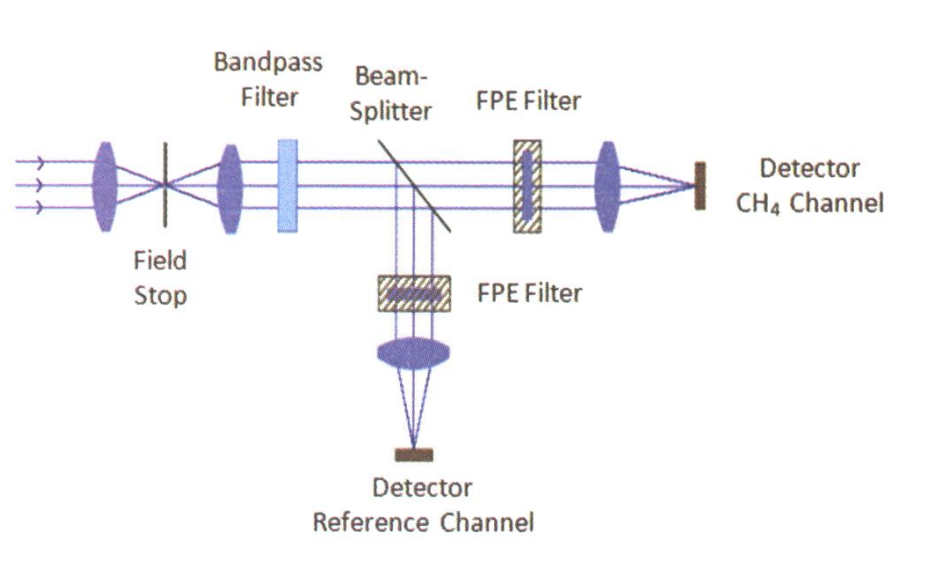
\includegraphics[scale=0.3]{methane sensor mars.png}
%\end{wrapfigure}


\subsection*{Βιβλιογραφία}
\begin{itemize}
\item[.] \url{https://en.wikipedia.org/wiki/Michelson_interferometer#Fourier_transform_spectrometer}
\item[.] (I.  ) \url{https://www.ligo.caltech.edu/page/ligos-ifo}
\item[.] (II. ) \url{https://pubmed.ncbi.nlm.nih.gov/23759857/}
\item[.] (IV.) \url{https://www.jstor.org/stable/24905819}


\end{itemize}
\end{document}